\documentclass[11pt]{article}
\usepackage[margin=1in]{geometry}
\usepackage{amsmath,amssymb}
\usepackage{enumitem}
\usepackage{tikz}
\usetikzlibrary{positioning}
\usepackage{fancyhdr}
\setlength{\headheight}{14pt}

\pagestyle{fancy}
\fancyhf{}
\lhead{Assignment 1, COMPSCI 683: Artificial Intelligence}
\rhead{Summer 2026}
\cfoot{\thepage}

\setlength{\parindent}{0pt}
\setlength{\parskip}{0.6em}

\begin{document}

\begin{center}
    {\Large \textbf{University of Massachusetts, Amherst}}\\[0.4em]
    {\large \textbf{CICS}}\\[0.8em]
    {\Large \textbf{COMPSCI 683: Artificial Intelligence}}\\[0.4em]
    {\large \textbf{Assignment 1: Uninformed Search}}
\end{center}

\begin{enumerate}[leftmargin=*, label=\textbf{\arabic*.}]

\item \textbf{(20 points)} A boolean satisfiability problem is given by a set of variables $x_1,\ldots,x_n$ (or their negations), organized into OR clauses. The clauses are connected by ANDs. This structure is known as Conjunctive Normal Form (CNF).

Consider the following example ($\vee$ stands for logical OR, and $\wedge$ stands for logical AND) that is a CNF formula with two clauses: $C_1=(x_1\vee x_3\vee x_4)$ and $C_2=(\neg x_1\vee x_2\vee \neg x_3)$:
\[
\phi(x_1,x_2,x_3,x_4)=C_1\wedge C_2=(x_1\vee x_3\vee x_4)\wedge(\neg x_1\vee x_2\vee \neg x_3).
\]

In order for the formula $\phi$ to be true, both clauses must be true. In order for $C_1$ to be true, we must have that $x_1=\text{true}$, $x_3=\text{true}$ or $x_4=\text{true}$; in order for $C_2$ to be true, we must have that $x_1=\text{false}$, $x_2=\text{true}$ or $x_3=\text{false}$.

A truth assignment is a setting of all the variables $x_1,\ldots,x_n$ to either true or false. A partial truth assignment is one where some variables unspecified, i.e. they do not have a true or false value. In the example above, setting $x_1=\text{true}$, $x_2=\text{false}$ with $x_3,x_4$ not set is a partial truth assignment.

A truth assignment is satisfying if every clause has at least one literal (that is, either $x_i$ or $\neg x_i$) that evaluates to true. In that case, the formula evaluates to true. Our objective is to find a satisfying, complete (i.e. not partial) truth assignment to a general $n$-variable boolean formula $\phi$ by searching. We start with all variables unspecified. At each iteration, we select some unspecified variable, and set its value to either true or false.

\begin{enumerate}[label=(\alph*), leftmargin=2em]
    \item \textbf{(5 points)} Give the representation of a state in this problem;
    \item \textbf{(5 points)} Using the state representation defined above, specify the initial state and goal states.
    \item \textbf{(5 points)} Define its actions and transition model.
    \item \textbf{(5 points)} What is the size of the search space when there are $n$ variables? That is, how many states does it have?
\end{enumerate}

\subsection*{Solution:}

\textbf{a)}

A boolean satisfiability problem is given by a set of variables $x_1, x_2, x_3, \dots, x_n$.

We can write a state as an n-tuple:
\[s = (v_1, v_2, v_3, \dots, v_n) \qquad \text{ where } v_i \in \{true, false, unspecified\}\]

\textbf{b)}

Initial State:
\[s_0 = (unspecified, unspecified, unspecified, \dots, unspecified) \qquad |s_0| = n\]

Goal State:
\[s = (v_1, v_2, v_3, \dots, v_n) \qquad \text{ where } v_i \in \{true, false\}\]

and this assignment satisfies $\phi.$

\textbf{c)}

Action:
\[Assign(x_i, b) \qquad \text{ where } x_i \text{ is unspecified and } b \in  \{true, false\}\]

Transition model:
\[T(s, Assign(x_i, b)) = (v_1, v_2, v_3, \dots,v_{i - 1} ,b , v_{i + 1}, \dots, v_n)\]

\textbf{d)}

For each variable, we have \{true, flase, unspecified\}

Search Space:
\[3^n\]

\newpage

\item \textbf{(20 points)} We are given a search problem where the minimal goal depth is $d$ and the branching factor is a finite value $b\ge 2$. Formally prove that the BFS algorithm terminates in at most $O(b^d)$ time. We assume that the only operations that take time is exploring a node (not placing it in the frontier), and that each such action takes one time step. You must prove this claim from first principles; in other words, you may not simply say that we have argued this in class and therefore the claim is true.

\subsection*{Solution:}

From the fact that the minimum goal depth is $d$, we know that there are no goal nodes from depth $0$ to depth $d-1$, while depth $d$ contains at least one goal node.

By the properties of BFS, before it explores the first goal node, it will not explore any node at depth $d+1$. Therefore, BFS will only explore all nodes from depth $0$ to depth $d$.

At depth $0$, the number of node: 
\[b^0 = 1\]

At depth $1$, the number of nodes:
\[b^1 = b\]

At depth $k$, the number of nodes:
\[b^k\]

BFS will only explore all nodes from depth $0$ to depth $d$.
\[\sum_{k=0}^{d}b^k = 1 + b + b^2 + \dots + b^d = \frac{b^{d+1} - 1}{b - 1}\]

Since $b \ge 2:$
\[\frac{b^{d+1} - 1}{b - 1} \le \frac{b}{b-1}b^d \le 2b^d\]

Thus the number of explored nodes is at most $2b^d$. By the assumption in the problem, each node exploration takes one time step.

Therefore the total running time of BFS is at most $2b^d$, which is $\mathcal{O}(b^d)$.





\newpage
\item \textbf{(20 points)} Iterative lengthening search is an iterative analogue of uniform-cost search (UCS). We set an increasing limit $\ell$ on path cost. Initially, $\ell=0$. We explore nodes in the same way we would under UCS. At iteration $t$, if a node is explored whose path cost exceeds the current limit, it is immediately discarded (we add it to a list of discarded nodes $D_t$). For each new iteration, the limit $\ell$ is set to the lowest path cost of any node discarded in the previous iteration, i.e., $\ell=\min\{g(n):n\in D_t\}$, if $D_t\ne \emptyset$, and remains the same otherwise.

\begin{enumerate}[label=(\alph*), leftmargin=2em]
    \item \textbf{(6 points)} Show that iterative lengthening search is optimal for general path costs. You may assume that all costs are integers (this is not a loss of generality if the search space is finite). You may wish to consider the minimal path cost $C$; what happens when we set the limit to be $\ell<C$?
    \item \textbf{(7 points)} Consider a uniform tree with branching factor $b$, solution depth $d$, and unit step costs (each action costs one unit). How many iterations will iterative lengthening require in the worst case?
    \item \textbf{(7 points)} Now consider the case where each step cost is a randomly chosen real number from the interval $[\varepsilon,1]$ for some $0<\varepsilon<1$. How many iterations are required in the worst case? Try to derive the best estimate you can.
\end{enumerate}

\subsection*{Solution}

\textbf{a)}

Let $C$ be the optimal path cost.

If current limit $\ell < C$, there is no possible the algorithm will return a solution with cost $< C$, because no such solution exists.

At each iteration, the new limit $\ell$ wil be the smallest path cost in the discarded nodes:
\[\ell = min\{g(n): n \in D_t\}\]

 So the limits increase in the same order as path costs, just like UCS. Since costs are integers, the limit will eventually reach $\ell = C$. The algorithm explores all nodes with path cost at most C. The first goal found has cost C, so it is optimal.

\textbf{b)}

With unit step costs, path cost equals depth.

The limit be will be: $0 \rightarrow 1 \rightarrow 2 \rightarrow \dots \rightarrow d$.

The solution found when $\ell = d$.

Worst Case:
\[d+1\]

\textbf{c)}

Assume $C$ is the optimal path cost.

Each step cost in $[\epsilon , 1]$, path costs may all be distinct. In the worst case it may require one iteration for each distinct path cost below or equal to the optimal cost C.

Since the solution is at depth $d$:
\[C \le d\]

Every path of depth $k$ at least have $k\epsilon$.

Thus,
\[k\epsilon \le C\]
\[k\le \frac{C}{\epsilon} \le \frac{d}{\epsilon}\]

The number of node at most:
\[\sum_{k=0}^{\frac{d}{\epsilon}} b^k = \mathcal{O}(b^{\frac{d}{\epsilon}})\]

worst Case:
\[\mathcal{O}(b^{\frac{d}{\epsilon}})\]




\newpage

\item \textbf{(20 points)} We have seen various search strategies, and analyzed their worst-case running time. Prove that any deterministic search algorithm will, in the worst case, search the entire state space. More formally, we define a search problem by a finite set of states $S$, a set of actions $A$, and a cost function $c:S\times A\times S\to\{1,\infty\}$ (i.e. the cost is uniform, but some states cannot be reached from some others, or equivalently have a cost of $\infty$), and a starting state $s_0\in S$. We assume that every state $s\in S$ is reachable from $s_0$, i.e. that there is a sequence of actions one can take from state $s_0$ such that one reaches the state $s$ after performing this sequence of actions, and such that the cost of reaching $s$ is finite. Prove the following theorem.

\textbf{Theorem 1.} Let Alg be a complete, deterministic uninformed search algorithm. Then for any search problem, there exists some choice of a state $s^*\in S$ such that Alg checks every state in $S$.

\subsection*{Solution:}

Since Alg is a deterministic, uninformed search algorithm, for a given search problem, it explore states in a fixed order:
\[
s_1, s_2, \ldots, s_m
\]
Since Alg is complete, and every state in $S$ can be reached from $s_0 \text(start)$, no matter which state in $S$ is chosen as the goal state, Alg must and can find it.

Thus, Alg will eventually explore every state in $S$. Assume $s^*$ be the last state explored.

Now choose $s^*$ as the goal state. Then all states explored earlier are not the target, so Alg will continue running until it reaches $s^*$. Therefore, Alg will explore all states in $S$.

Thus, there exists a goal state $s^* \in S$ such that the algorithm will explore the entire state space.

Therefore, in the worst case, the algorithm will explore every state in $S$.


\newpage

\item \textbf{(20 points)} Consider the graph shown in Figure~\ref{fig:routes}. Let $S$ be the initial state and $G$ be the goal state. The cost of each action is as indicated.

\begin{figure}[h]
\centering
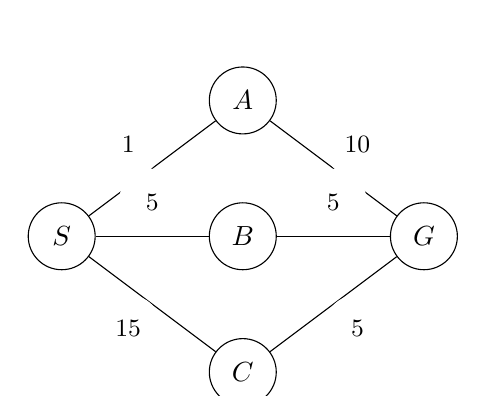
\begin{tikzpicture}[scale=1.15, every node/.style={circle, draw, minimum size=0.85cm}, edge label/.style={draw=none, fill=white, inner sep=1pt, font=\small}]
    \node (S) at (0,0) {$S$};
    \node (A) at (2,1.5) {$A$};
    \node (B) at (2,0) {$B$};
    \node (C) at (2,-1.5) {$C$};
    \node (G) at (4,0) {$G$};

    \draw (S) -- node[edge label, above left] {$1$} (A);
    \draw (A) -- node[edge label, above right] {$10$} (G);
    \draw (S) -- node[edge label, above] {$5$} (B);
    \draw (B) -- node[edge label, above] {$5$} (G);
    \draw (S) -- node[edge label, below left] {$15$} (C);
    \draw (C) -- node[edge label, below right] {$5$} (G);
\end{tikzpicture}
\caption{Graph of routes between $S$ and $G$.}
\label{fig:routes}
\end{figure}

\begin{enumerate}[label=(\alph*), leftmargin=2em]
    \item \textbf{(8 points)} Give a trace of uniform-cost search, assuming we run a graph search; you may implement UCS and submit the program trace.
    \item \textbf{(12 points)} When UCS generates $G$ which is the goal with a path cost of 11, why doesn't the algorithm halt and return the search result since the goal has been found? Using this observation, prove the following claim (also shown in class)

    \textbf{Theorem 2.} For any search problem, UCS returns an optimal goal state.
\end{enumerate}

\end{enumerate}

\subsection*{Solution:}

\textbf{a)}

\text{1) Initial State:}

frontier = $\{(S, 0)\}$

\text{2) Step 1:}

Pop $S$

frontier = $\{(A, 1), (B, 5), (C, 15)\}$

\text{3) Step 2:}

Pop $A$

frontier = $\{(B, 5), (G, 11), (C, 15)\}$

\text{4) Step 3:}

Pop $B$

frontier = $\{(G, 10), (C, 15)\}$

\text{5) Step 4:}

Pop $G$, goal state

frontier = $\{(C, 15)\}$

\text{6) Solution:}

Path: $S \rightarrow B \rightarrow G$

Cost: 10

\textbf{b)}

UCS stops only when the goal is popped from the frontier, not when it is generated.

At Step 2, the frontier still have $(B, 5)$ and $B$ may lead to cheaper cost, which is 
\[S \rightarrow B \rightarrow G \qquad 5 + 5 = 10 < 11\]

Thus, UCS do not return $(G, 11)$.

\textbf{Proof}

Assume the contradiction that there is a better goal $G'$ with cost $C' < C$.

Then along the path to $G'$, there must be some frontier node with path cost less than or equal to $C'$. Hence that node has cost $< C$.

But UCS would have removed that lower-cost node before removing G, contradiction.

Therefore no cheaper goal exists, so UCS returns an optimal goal state.
\end{document}
